\documentclass[10pt,final,journal,letterpaper,oneside,twocolumn]{IEEEtran}

\usepackage{fix2col}
\usepackage{graphicx}
\usepackage{tikz}
\usetikzlibrary{arrows.meta,
  shapes.geometric,
  shapes.misc,shapes.arrows,
  snakes,patterns}
\usepackage{tikzinclude}
\usepackage{subcaption}
\usepackage{multirow}

\usepackage[english]{babel}

\usepackage{amsmath}
\usepackage{amssymb}
\usepackage{bm}
\usepackage{mathrsfs}
\usepackage{bbm}
\usepackage{cleveref}

\usepackage{lipsum}

\newcommand{\Real}{{\rm I\!R}}

\newcounter{mytempcntr}

\title{Dynamics \& Control of Closed Kinematic Chains}
\author{Nidish Narayanaa Balaji\\S01276643\thanks{Course Project,
    MECH520, Dec 2018}}
\markboth{MECH 508, Aug-Dec 2018}{Nidish: Dynamics and Control of CKC}
\begin{document}
\maketitle{}

\begin{abstract}
  The dynamics and control of closed kinematic chains is considered in
  the current study. The systems are posed as differential algebraic
  systems and modeled using singular perturbations. Standard results
  are invoked in order to prove (a) that the singularly perturbed
  systems represent the original system (within a bounded error), and
  (b) the system may be controlled using the proposed control
  laws. Results are presented for both regulation as well as tracking
  control.
\end{abstract}
\begin{IEEEkeywords}
  Closed Kinematic Chains, Differential Algebraic Equations, Singular
  Perturbations, Lyapunov Stability
\end{IEEEkeywords}

\section{Introduction and Motivation}
\label{sec:intr-motiv}

Kinematic chains or linkages are classical examples of systems with
holonomic constraints. They consist of component ``links'' in
$\Real^2$ (planar mechanisms) or $\Real^3$ (spatial
mechanisms) statically constrained together through joints or
``kinematic pairs''~\cite{ghosh1988theory}. Mathematically represented
as additional algebraic equations, the constraints dictate the
effective number of Degrees-Of-Freedom (DOFs) such a system has. In
their primitive forms, these are classified as
Differential-Algebraic-Equations (DAEs), since the systems are modeled
with differential equations governing their dynamics and algebraic
equations representing their constraints. 

Among DAEs, there are some cases where the constraints may be solved
analytically in terms of a minimal number of DOFs (equal to the
effective DOFs of the system). Here, the DAE may be represented
exactly by a reduced set of Ordinary Differential Equations
(ODEs). Open Kinematic Chains (OKCs) are examples where this is
possible. However, this is not possible in the most general case,
wherein the system can not be represented exactly in terms of a
minimal number of DOFs. Here, however, local maps may be constructed
between DAE in terms of the ``dependent generalized coordinates'' and
an ODE in terms of a minimal ``independent generalized
coordinates''~\cite{ghorbel_modeling_2000}. As expected, multiple
choices are possible for the latter set, leading to representational
differences. There exist several studies in the literature such as
\cite{ghorbel_modeling_2000, gunawardana_reduced_nodate}, where the
definition and existence of such maps are established.

Kinematic chains in which there exist one or more loops, referred to
as Closed Kinematic Chains (CKCs) henceforth, are a classical example
of such systems, where the constraints may not be solved analytically
and the system dynamics may be expressed only in a local sense. The
current work deals with the set-point and tracking control of such
systems. A singular perturbation formulation is employed for modeling
the system as in~\cite{dabney_modeling_2002}, since this allows for
the application of classical stability theorems. Starting with the
formulation of the system, the singularly perturbed system is shown to
be representative of the original DAE, followed by the definitions of
the control systems and proofs of convergence for the set-point and
tracking cases.

\section{Problem Definition}
\label{sec:problem-definition}

Denoting the dependent generalized coordinates as $q'\in \Real^n$, the
original DAE is represented by the system
\begin{align}
  \bm{D}'(q')\ddot{q}' + \bm{C'}(q', \dot{q}')\dot{q}' + h'(q') &=
                                                         u'(t)\nonumber\\
  \phi(q') &= 0,
  \label{eq:DAE}
\end{align}
where $\bm{D}'(q'), \bm{C}'(q', \dot{q}') \in \Real^{n\times n}$
represent the inertia and Christoffel symbols matrices respectively;
$h'(q') \in \Real^n$ the ``gravity vector''; $u'(t) \in \Real^n$ the
forcing/control impulse; and $\phi(q') \in \Real^{n-d}$ the set of
algebraic constraints. Since the current work deals with CKCs, the
choice of independent generalized coordinates $q\in \Real^d$ may be
made such that $q\subset q'$. $q'$ is reordered as
\begin{equation}
  q' = \begin{bmatrix} q\\ z \end{bmatrix},
  \label{eq:qreord}
\end{equation}
where $z\in \Real^{n-d}$ represents the rest of the coordinates in
$q'$. Using the generalized coordinates of the component OKCs in the
system, the set $q'$ becomes a set of link angles required to uniquely
specify the configuration of the component OKCs, and $q$ becomes a set
of $d$ link angles in those.

Augmenting this choice along with the constraint equations yields a
function
\begin{align}
  \Psi(q', q) &= \begin{bmatrix} \phi(q')\\ \begin{bmatrix} \bm{I}_{d\times d}
      & \bm{0}_{d\times
        (n-d)} \end{bmatrix}q' - q\end{bmatrix}\nonumber\\
  \Psi&: \Real^n \times \Real^d \to \Real^n.
  \label{eq:Psi} 
\end{align}
For the constraints to hold, $\Psi(q', q) = 0$ has to be ensured at
each point during simulation. As in~\cite{ghorbel_modeling_2000}, for
developing a reduced model in terms of the independent generalized
coordinates $q$, the Implicit Function Theorem (IFT) is invoked on
this function to establish sufficient conditions for the existence of
a map $\sigma: \Real^d \to \Real^n$ defining
\begin{equation}
  q' = \sigma(q)
  \label{eq:map}
\end{equation}
as the mapping between the dependent and independent generalized
coordinates. Part of the requirements for this result is that the
Jacobian $\Psi_{q'}$ be non-singular~\footnote{the others, concerning
  the smoothness of the function, are all assumed to be valid for the
  current applications}. This also provides the derivative matrix $\rho:
\Real^n \times \Real^d  \to \Real^{n\times d}$ 
\begin{equation}
  \dot{q}' = \rho(q', q) q =
  \underbrace{-\Psi_{q'}^{-1}\Psi_q}_{\rho(q', q)} q.
  \label{eq:dermap}
\end{equation}
The ``workspace'' of the original system is defined by $\mathcal{U}'
\triangleq \{q'\in \Real^n: \phi(q') = 0\} \subseteq
\Real^n$. Physically, this is the sub-domain where the constraints are
fully valid. The differential equation part of the DAE alone is
sufficient to describe the system on this subspace. Following the
above parametrization, a ``non-singular workspace'' is defined as
$\mathcal{V}' \triangleq \{q'\in \mathcal{U}': \Psi_{q'} \neq 0\}
\subseteq \mathcal{U}'$. Physically, this represents the domain
wherein a ``reduced'' formulation of the system is definitely valid
(domain of validity of the IFT~\footnote{It must be noted that the IFT is only a sufficient
  condition for the existence of the maps. Singularity of the Jacobian
  alone need not imply anything.}), i.e., the system may be
represented locally using exactly $d$ independent generalized
coordinates ($q$). A configuration $q'$ is said to be singular if
$q'\in \mathcal{U}'$ but $q' \notin \mathcal{V}'$, i.e., $\Psi_{q'} =
0$. This could imply either that the system can not be defined at all,
or that the choice of the generalized coordinates is questionable for
the given $q'$.

Using the above mappings, it is possible to
define~\cite{ghorbel_modeling_2000} a reduced system in a sub-space of
$\mathcal{W'}\subseteq \mathcal{V}'$ (where the maps exist) as a set
of $d$ ordinary differential equations:
\begin{align}
  \bm{D}(q')\ddot{q} + \bm{C}(q', \dot{q}')\dot{q} &+ h(q) =
  u(t)\nonumber\\
  \bm{D} &= \rho^T\bm{D}'\rho\nonumber\\
  \bm{C} &= \rho^T\bm{D}'\dot{\rho} + \rho^T\bm{C}'\rho\nonumber\\
  h &= \rho^T h'\nonumber\\
  u &= \rho^T u'.
  \label{eq:redmod}  
\end{align}

\subsection{Singular Perturbation Formulation (SPF)}
\label{sec:sing-pert-form}

A ``singularly perturbed'' dynamical system is defined as follows:
\begin{align}
  \bm{D}\ddot{q} + \bm{C}\dot{q} + h(q) &= u(t)\nonumber\\
  \epsilon \dot{w} &= s(q, w).
  \label{eq:spert0}
\end{align}
When the terms are appropriately scaled, $\epsilon$ represents the
ratio of time-scales associated with the dynamics of $q$ and $w$. For
small $\epsilon$, the dynamics of $w$ becomes infinitely faster
relative to that of $q$ and the second equation in effect becomes the
algebraic constraint $s(q, w) = 0$. As in~\cite{wange_domain_2004},
the choice for the fast dynamics is $\dot{w} = -w/\epsilon $, with
$w=\phi(q')$. Writing this in terms of the
parameterization in~\cref{eq:qreord} defines the singularly perturbed
system as,
\begin{align}
  \bm{D}(q, z)\ddot{q} + \bm{C}(q, z, \dot{q}, \dot{z})\dot{q} + h(q,
  z) &= u(t)\nonumber\\
  \dot{z} = -\phi_z^{-1}(q, z)\phi_q(q, z)\dot{q} &-
            \frac{1}{\epsilon}\phi_z^{-1}(q, z)\phi(q, z).
  \label{eq:spertsys}
\end{align}
In assessing the accuracy of the singularly perturbed system in
representing that original DAE, the local form of Tikhonov's
theorem~\cite{khalil2002nonlinear} may be invoked. Representing the
dynamics of the states $x={\begin{bmatrix} q&
    \dot{q} \end{bmatrix}}^T$ by $f(t, x, z, \epsilon)$, and that of
the singular perturbation with respect to the variables $z$ by the
function $g(t, x, z, \epsilon)$ as
\begin{align}
  \dot{x} &= f(t, x, z, \epsilon)\nonumber\\
  \epsilon\dot{z} &= g(t, x, z, \epsilon).
  \label{eq:spertform}                    
\end{align}
For a given solution $\bar{x}(t)$ of the original DAE, the solution in
$z$ is given by the solution of the algebraic equation as $h(t,
\bar{x})$. The ``fast dynamics'' of the system is retrieved by writing the
equations in terms of the fast time-scale $\tau=t/\epsilon$ as 
\begin{align}
  \frac{dx}{d\tau} &= \epsilon f(t, x, z, \epsilon)\nonumber\\
  \frac{dz}{d\tau} &= g(t, x, z, \epsilon).
  \label{eq:fasttime}
\end{align}
Transforming this into the error coordinates $y-h(t, \bar{x})$, the
dynamics is given by
\begin{align}
  \frac{dy}{d\tau} &= g(t, x, y+h, \epsilon) - \frac{\partial
    h}{\partial t} - \epsilon f(t, x, z, \epsilon) \nabla_{\bar{x}}
                     h(t, \bar{x}).
  \label{eq:bdyn}                     
\end{align}
Setting $\epsilon=0$ gives the ``boundary layer'' system
\begin{equation}
  \label{eq:blsys}
  \frac{dy}{d\tau} = g(t, x, y+h, 0) = -\phi_z^{-1}(q, y+h)\phi(q, y+h).
\end{equation}
If the origin of this system is uniformly exponentially stable
(locally), Tikhonov's theorem guarantees that for $t \in [t_0, t_1]$,
it is possible, given $t_b\in (t_0, t_1)$, to obtain $\epsilon^*(t_b,
t_1)$ such that the error between the original and perturbed systems
are of order $\mathcal{O}(\epsilon)$ for time $t\in
(t_b, t_1]$ when $0< \epsilon< \epsilon^*$. The exponential stability
of the origin may be concluded by if the eigen values of the
corresponding Jacobian are all in the left half of the s-plane
(Real-Imaginary plane)~\cite{gordon_singular_1998}, i.e.,
\begin{equation}
  \Re\{\lambda\{\nabla_y g(t, x, y+h, 0)\}\} \leq
  \Re\{\lambda\{\nabla_y \phi_z^{-1}\phi \}\} \leq c \leq 0.
  \label{eq:expstabor}
\end{equation}
Hence, $x-\bar{x} = \mathcal{O}(\epsilon)$ \& $z-h(t, \bar{x}) =
\mathcal{O}(\epsilon)$ for $t\in (t_b, t_1]$. As
in~\cite{wang_domain_2004}, it may also be shown that if an
appropriate controller $u(t)$ is chosen to track a desired trajectory
$x_d(t)$ such that the functions $f, g, h$ \& their partial
derivatives bounded (in local compact domains in $x$ \& $y$, $t>0$ in
$t$, and $\epsilon\in (0, \epsilon_0]$) and ensuring that the desired
trajectory is tracked for the original DAE, the infinite time
(uniform) version of Tikhonov's theorem will be applicable to
demonstrate the accuracy (stability) of the singularly perturbed
system in approximating the solution of the original DAE.

It must be noted that $\phi_z$ becomes singular for the singular
configurations of the system, rendering the perturbation dynamics
in~\cref{eq:spertsys} undefined. Thus, the singularly perturbed form
of the dynamical system approximates the original system as long as
the system stays sufficiently away from singular configurations in the
work-space, in addition to the conditions noted
above. Quoting~\cite{gordon_singular_1998}, ``this limitation reflects
the local nature of general nonlinear inversion methods which are used
in all DAE solution methods''.

Additionally, the domain of validity of the SPF model may be shown to
be a superset of the non-singular work-space $\mathcal{V}'$~\cite{wang_domain_2004}. 
\subsection{Set-Point Control}
\label{sec:set-point-control}
\begin{figure*}[!h]
  \centering
  \includetikzgraphics[5bar]{FIGS/diags}
  \caption{Schematic of the 5-bar CKC with two 2-bar component
    OKCs. $w_1$ \& $w_2$ represent the two kinematic loop-closure
    constraint terms that will be set to zero.}
  \label{fig:schem5}
\end{figure*}

Set-point control for fully known parameters is fairly trivial since a
PD control with simple gravity compensation may be used to guarantee
uniqueness and local asymptotic stability. The controller, in terms of
the independent generalized coordinates, is given by
\begin{equation}
  u(t) = \bm{K}_P\underbrace{(q_d-q)}_{\tilde{q}} - \bm{K}_V\dot{q} +
  h(q_d)
  \label{eq:setptctrl}
\end{equation}
Since the nonlinear vector $h(q)$ is conservative in nature (arising
from a potential), its potential function is defined, and is denoted
by $V(q)$. Using a candidate function $\mathcal{V} =
\frac{1}{2}\dot{q}^T\bm{D}(q)\dot{q} + V(q) + \tilde{q}^Th(q_d) +
\frac{1}{2}\tilde{q}^T\bm{K}_P\tilde{q} $. The positive definiteness
of this candidate function depends on the positive definiteness of the
hessian term $\frac{\partial h}{\partial q}(q) + \bm{K}_P$. When
$h(q)$ is Lipschitz and its gradient is bounded by $M_1$, gains in the
diagonal matrix $\bm{K}_P$ may be chosen such that $k_{pi} >
M_1$. This makes the function a valid Lyapunov candidate. The
equilibria of the controlled system are the solutions of the algebraic
equation,
\begin{equation}
  h(q_d) - h(q) = \bm{K}_P(q_d-q).
\end{equation}
The above condition on the gains of $\bm{K}_P$ are sufficient to
conclude that the only solution of this is $q=q_d$.

The time derivative of the Lyapunov function becomes
\begin{equation*}
  \dot{\mathcal{V}} = -\dot{q}^T\bm{K}_v\dot{q}.
\end{equation*}
Choosing a positive definite matrix $\bm{K}_v$ makes
$-\dot{\mathcal{V}} \geq 0$. The set where $\dot{\mathcal{V}}=0$ is
satisfied is $\dot{q}=0$, which corresponds to only equilibrium of the
system, $q=q_d$. Hence, La Salle's theorem becomes
applicable~\cite{vidyasagar1978nonlinear} and it is shown that the
controlled system is uniformly asymptotically stable about the point
$\begin{bmatrix} q_d & 0 \end{bmatrix}$.

Two points must be made here regarding the above results: (1) The
uniqueness of the equilibrium of the controlled system (after tuning
the gains sufficiently), is guaranteed only if the derivative
$\frac{\partial h}{\partial q}$ exists and is bounded. This, in turn,
is true only when the mapping $\sigma(.)$ exists between $q$ \&
$q'$. (2) All the results above, on account of being described based
on locally defined dynamics, are only valid locally, as long as the
system is sufficiently removed from the singular regions.

\subsection{Tracking Control}
\label{sec:tracking-control}
Denoting the desired trajectory with $q_d(t), \dot{q}_d$ in terms of
the independent generalized coordinates, the controller used
in~\cite{wang_control_2006} is given by
\begin{align}
  u(t) = \bm{D}(q, z)a + \bm{C}(q, \dot{q}, &z, \dot{z})v + h(q) -
  \bm{K}_Dr\nonumber\\
  \tilde{q}(t) \triangleq q(t)-q_d(t)\quad &r=\dot{\tilde{q}} +
  \bm{\Lambda} \tilde{q}\nonumber\\
  v = \dot{q}_d-\bm{\Lambda}\tilde{q}\quad &a=\dot{v}.
  \label{eq:trackctrl}
\end{align}
Substituting the above in the singularly perturbed equations, the
closed loop equations of motion becomes,
\begin{align}
  &\bm{D}(q, z)\dot{r} + \bm{C}(q, \dot{q}, z, \dot{z})r + \bm{K}_Dr =
    0\nonumber\\
  &\dot{w} = -\frac{1}{\epsilon}w.\label{eq:trackclloop}
\end{align}
Including the dynamics of $w$ in the system implies that the
state-space is represented by ${\begin{bmatrix} q & \dot{q} &
    w \end{bmatrix}}^T$. It must be noted that the derivatives of $w$
are not part of this state-vector. Choosing the function candidate
\begin{align}
  \mathcal{V}(t, q, \dot{q}, w) &= d_1V_1(t, q, \dot{q}, w) + d_2V_2(t,
                                  q, \dot{q}, w)\nonumber\\
                                &= d_1\left( \frac{1}{2}r^T\bm{D}r +
                                  \tilde{q}^T \bm{\Lambda}^T \bm{K}_D
                                  \tilde{q} \right) +\nonumber\\
                                & \qquad\qquad\qquad
                                  d_2\left(\frac{1}{2}w^T\bm{M} w
                                  \right),
  \label{eq:lyapcand}
\end{align}
where $\bm{M}$ is some constant, diagonal, positive definite matrix,
the properties are first established below. Since the current study
deals with CKCs whose component OKCs all have bounded inertia
matrices, $\bm{D}'$ is bounded. Since $\bm{D} = \rho^T\bm{D}'\rho$,
matrix $\bm{D}$ is bounded as long as the trajectory stays away from
singular configurations. The other parts of the function are each
positive definite since they are quadratic in their components with
constant, positive definite weights. Thus, the function candidate
$\mathcal{V}(.)$ is a suitable candidate for Lyapunov stability
analysis of the controlled system. The first time derivative of the
function is given as
\begin{align}
  \dot{\mathcal{V}}(t, q, \dot{q}, w) &= d_1\left(\frac{1}{2}r^T
                                        (\dot{\bm{D}} - 2\bm{C})r
                                        -r^T\bm{K}_Dr
                                        -2\dot{\tilde{q}}^T
                                        \bm{\Lambda} \bm{K}_D\tilde{q}
                                        \right)\nonumber\\
                                      &- \frac{d_2}{\epsilon}\left(
                                        w^T\bm{M}w \right)\nonumber\\
  &= -d_1\dot{\tilde{q}}^T\bm{K}_D\dot{\tilde{q}} -d_1
    \tilde{q}^T\bm{\Lambda}^T \bm{K}_D \bm{\Lambda} \tilde{q} -
    \frac{d_2}{\epsilon} w^T \bm{M} w.
  \label{eq:lyapdot}
\end{align}
It can be observed that $-\dot{\mathcal{V}}$ is locally positive
definite. Hence, the equilibrium of the closed loop system $(q_d(t),
\dot{q}_d(t), w=0)$ is locally asymptotically
stable~\cite{vidyasagar1978nonlinear}. Further, invoking the results
from~\cref{sec:sing-pert-form}, it is recalled that stability of the
perturbed system implies stability of the original DAE system.

\subsection{Model Description}
\label{sec:model-description}

\Cref{fig:schem5} represents a schematic view of the 5-bar mechanism
to be considered for the current study. Each link has mass $m_i$,
planar moment of Inertia $I_i$, link length $l_i$, and length from pin
to center of mass $c_i$ describing the equations of motion (see
\cref{sec:equations-motion} for exact expressions). The dependent and
the independent generalized coordinates are chosen as $q'
= \begin{bmatrix} \theta_1 & \theta_2 & \theta_3 &
  \theta_4 \end{bmatrix}^T$ and $q = \begin{bmatrix} \theta_1 &
  \theta_3 \end{bmatrix}^T$ respectively (giving $n=4$, $d=2$). As can
be observed, the CKC is formulated as consisting of two 2-bar OKCs: 
[Link 1-Link 2] and [Link 3-Link 4] respectively. Thus, the
loop-closure constraints $\phi(.): \Real^4 \to \Real^2$ giving
$\phi(q') = \begin{bmatrix} w_1 & w_2 \end{bmatrix}^T$ represent the
constraint of the end effector points from both the components to be
coincident. Since the mechanism is planar, this leads to the
corresponding two constraints.

\begin{table}[!h]
  \centering
  \caption{Specifications of the 5-bar mechanism}
  \begin{tabular}[!h]{lcccc}
    \hline
    & Length & CM & Mass & Inertia\\
    Link & $l_i$ & $c_i$ & $m_i$ & $I_i$\\
    \hline
    0 & 0.3048 & - & - & -\\
    1 & 0.2794 & 0.1466 & 0.2451 & $2.770\times 10^{-3}$\\
    2 & 0.3048 & 0.1581 & 0.2611 & $3.476\times 10^{-3}$\\
    3 & 0.3048 & 0.1467 & 0.2611 & $3.476\times 10^{-3}$\\
    4 & 0.2794 & 0.1410 & 0.2352 & $2.607\times 10^{-3}$\\
    \hline 
  \end{tabular}
  \label{tab:5barspec}
\end{table}

\Cref{tab:5barspec} gives the specifications that were used
in~\cite{ghorbel_modeling_2000} for the 5-bar mechanism, representing
the identified quantities for the Rice Planar Delta Robot (RPDR); the
same parameters will be used for the current investigation.

\section{Results and Discussions}
\label{sec:results-discussions}

\subsection{Singular Configurations}
\label{sec:sing-conf}

Since singularity of the matrix $\Psi_{q'}$ implies that a map from
the independent to the dependent generalized coordinates can no longer
be defined using the results from the classical IFT. The
configurations where this happens are traced out
in~\cref{fig:sing5}.

\begin{figure}[!h]
  \centering
  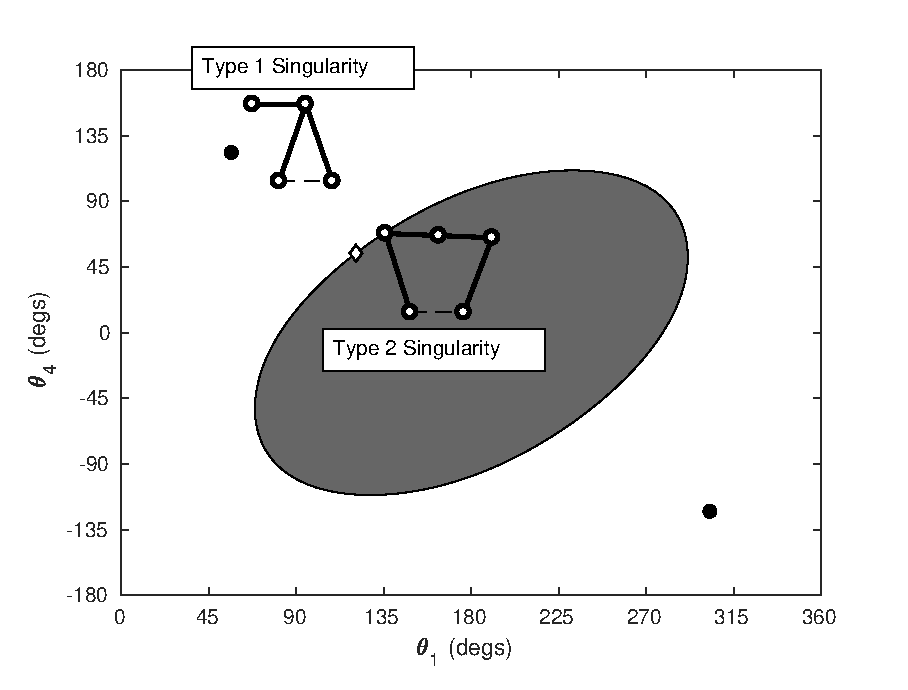
\includegraphics[width=\linewidth]{FIGS/SING5}
  \caption{Singular Configurations of the mechanism. Unreachable
    configurations are shaded gray.}
  \label{fig:sing5}
\end{figure}

It can be seen in this case that both these ``singularities'' result
in the mechanism getting locked onto a configuration wherein the
independent generalized coordinates are no longer strictly
independent. In the Type 1 singularity, $\theta_1$ \& $\theta_3$ get
``locked on'' to particular values, with links 2 \& 4 degenerating
into a pendulum-like behavior. In the Type 2 singularity, $\theta_1$
\& $\theta_3$ have a functional relationship represented by the closed
curve in the plot, reflecting the fact that links 2 \& 4 have locked
against each other in such a way as to make the mechanism effectively
4-bar. In both these singularities, the system ceases to have two DOFs
and becomes just single DOF systems. Type 1 singularity is represented
by just a single point since eventhough the system has a single DOF,
changes in configuration do not correspond to any changes in the
chosen generalized coordinates.

\subsection{Set-Point Control}
\label{sec:set-point-control-1}

\begin{figure*}[!h]
  \centering
  % \setcounter{mytempcntr}{\value{figure}}
  % \setcounter{figure}{3}
  \centering
  \begin{subfigure}[!t]{0.5\linewidth}
    \centering
    \includegraphics[width=0.7\linewidth]{./FIGS/SETPOINTOBJ}
    \caption{}
    \label{fig:setptobj}
  \end{subfigure}%
  \begin{subfigure}[!t]{0.5\linewidth}
    \centering
    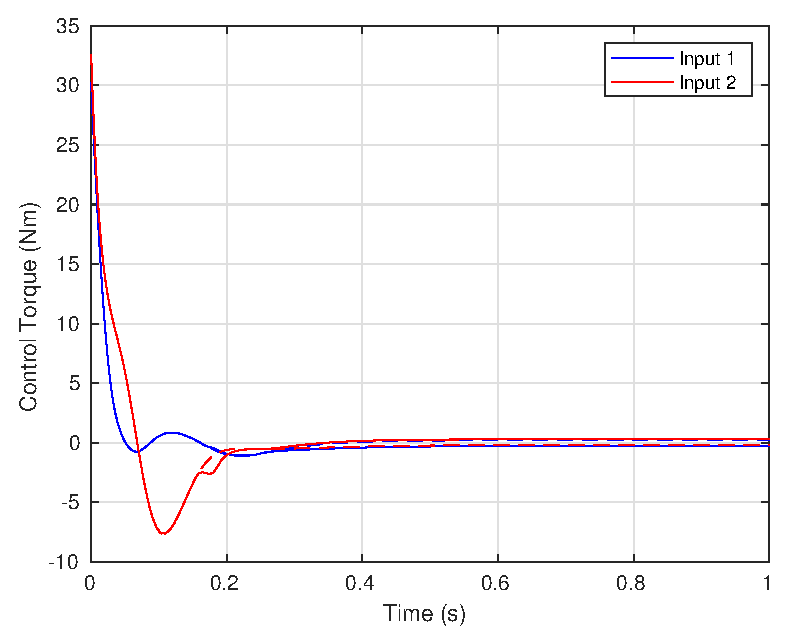
\includegraphics[width=0.7\linewidth]{./FIGS/SETPT_3}
    \caption{}
    \label{fig:setpt3}
  \end{subfigure}
  
  \begin{subfigure}[!t]{0.5\linewidth}
    \centering
    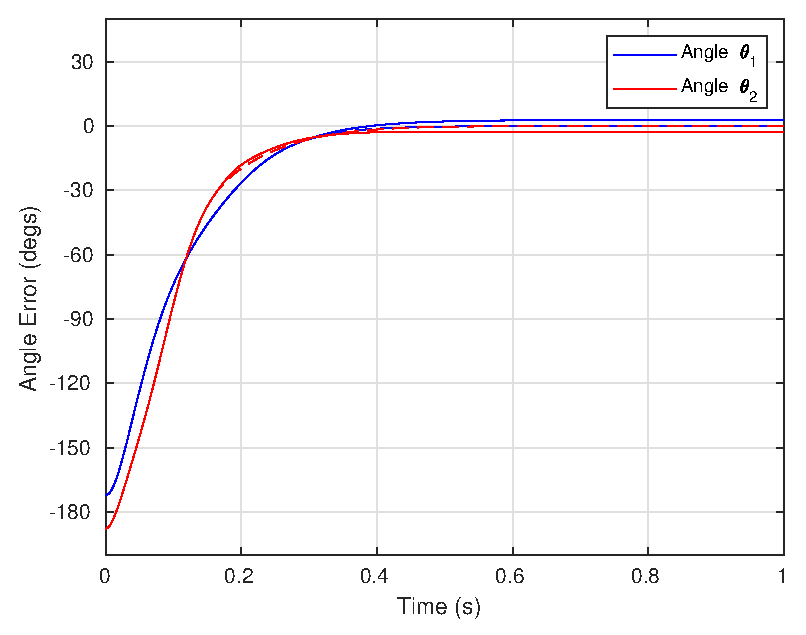
\includegraphics[width=0.7\linewidth]{./FIGS/SETPT_1}
    \caption{}
    \label{fig:setpt1}
  \end{subfigure}%
  \begin{subfigure}[!t]{0.5\linewidth}
    \centering
    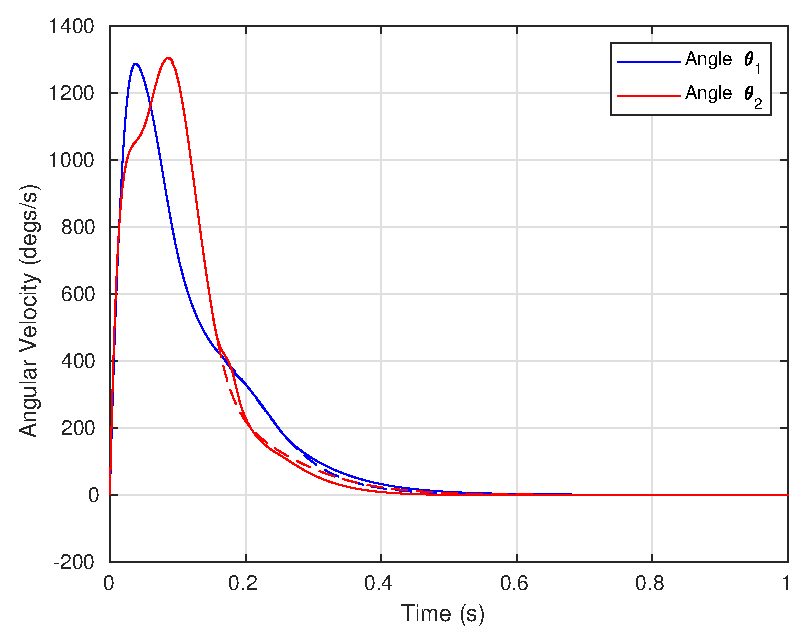
\includegraphics[width=0.7\linewidth]{./FIGS/SETPT_2}
    \caption{}
    \label{fig:setpt2}
  \end{subfigure}
  \caption{Set-Point Control Results. (a) represents the initial
    (blue) and desired (red) configurations, (b) shows the control
    torque time history, and (c-d) show the angular error and
    velocities for $\theta_1$ \& $\theta_3$. Dashed lines are
    simulations with the SPF; continuous lines are simulations with
    the reduced system.}
  \label{fig:setpoint}
  % \setcounter{figure}{\value{mytempcntr}}
\end{figure*}

\Cref{fig:setptobj} represents the initial configuration (which
happens to be a stable equilibrium for the system) in
\textcolor{blue}{blue} and the final configuration in
\textcolor{red}{red} for the set-point control test case. The
controller gains are chosen as
\begin{equation}
  \bm{K}_P = \begin{bmatrix} 10 & 0\\ 0 & 10 \end{bmatrix},
  \,\text{and}\,\,
  \bm{K}_v = \begin{bmatrix} 1 & 0\\ 0 & 1 \end{bmatrix}.
  \label{eq:setptgains}
\end{equation}
The gains were fixed based on the control impulses
(see~\cref{fig:setpt3}) not exceeding
$30Nm$ in the initial regime. \Crefrange{fig:setpt1}{fig:setpt2} show
the control performance in terms of the angle errors with respect to
both the angles $\theta_1$ \& $\theta_3$ as well as their
corresponding angular velocities $\dot{\theta}_1$ \&
$\dot{\theta}_3$. For the SPF simulations, the perturbation parameter
$\epsilon$ is fixed to be $10^{-3}$ based on trial and error in order
to give satisfactory accuracy with respect to the exact system. It can
be observed that as proven, the controller is effective in stabilizing
the system at the desired configuration. The simulations were
conducted using just the reduced model (as in~\cref{eq:redmod}) as
well as the SPF (as in~\cref{eq:spertsys}). A notable difference is
that the nonlinear mapping $\sigma(.)$ is not known analytically and a
nonlinear solver will have to be employed at each step for the reduced
model, while the SPF does not involve this cost at each time step: all
the link angles are already part of the state-space.

The reduced model results are plotted using continuous lines and the
SPF results are plotted using dashed lines in~\cref{fig:setpoint}. It
can be observed that the SPF follows the reduced model closely
throughout the simulation, serving additionally, as a demonstration
for the convergence results in~\cref{sec:sing-pert-form}.

\subsection{Tracking Control}
\label{sec:tracking-control-1}

For the tracking control, the desired trajectory is fixed in terms of
the independent generalized coordinates as
\begin{align}
  \theta_1^d(t) &= \frac{\pi}{3}\sin t\nonumber\\
  \theta_3^d(t) &= \frac{\pi}{4}(1-\cos t)
  \label{eq:trackdes}.
\end{align}
It was ensured that no kinematic singularities $\Psi_{q'}=0$ occurs
along the trajectory. Using the control law in~\cref{eq:trackctrl}
with the gain matrices fixed to
\begin{equation}
  \label{eq:trackgains}
  \bm{\Lambda} = \begin{bmatrix} 1.0 & 0\\0 & 1.0 \end{bmatrix}\,
  \text{and}\,
  \bm{K}_d = \begin{bmatrix} 10.0 & 0\\0 & 10.0 \end{bmatrix},
\end{equation}
simulations were carried out for the system. The initial condition was
fixed to be the stable equilibrium initial condition used for the
set-point control (see \textcolor{blue}{blue} configuration
in~\cref{fig:setptobj}). The singular perturbation coefficient
$\epsilon$ is fixed to $10^{-4}$ to give satisfactory accuracy over
the regime of interest. 

\Cref{fig:trackobj} depicts a configuration-space view of the response
of the system. Due to the choice of the objective, the desired
trajectory will be a closed ellipse here. It can be observed that
although the system starts from a completely different configuration,
the controller effectively makes the desired trajectory
convergent. \Cref{fig:track3} depicts the time histories of the
control impulses required for each torquer. Once again, the gains
above were fixed in such a manner that the maximal control impulse
does not exceed $30 Nm$ for the initial transients and $5Nm$ at steady
state operation. \Crefrange{fig:track1}{fig:track2} depict the time
histories of these quantities for one and a half cycles of
operation. It can be observed that the singularly perturbed form
exactly follows the desired trajectory, but the more exact reduced
model periodically sees some deviations, which are soon corrected by
the controller. This demonstrates a crucial aspect of the convergence
proof presented in~\cref{sec:tracking-control}, namely that the
stability result for the controller is applicable only for the
SPF. The original system ends up being stabilized on account of
Tikhonov's theorem assuring that the deviation between the SPF and the
DAE responses is always bounded to be within
$\mathcal{O}(\epsilon)$. Thus, using a controller whose stability is
established only for the SPF model can be used to effectively control
the original system.


\begin{figure*}[!h]
  \centering
  % \setcounter{mytempcntr}{\value{figure}}
  % \setcounter{figure}{3}
  \centering
  \begin{subfigure}[!t]{0.5\linewidth}
    \centering
    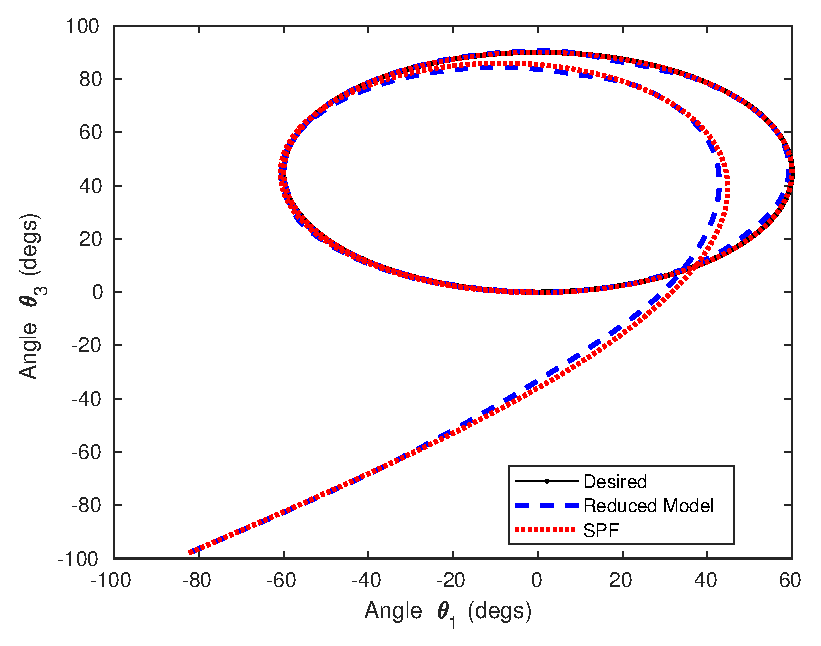
\includegraphics[width=0.7\linewidth]{./FIGS/TRACKOBJ}
    \caption{}
    \label{fig:trackobj}
  \end{subfigure}%
  \begin{subfigure}[!t]{0.5\linewidth}
    \centering
    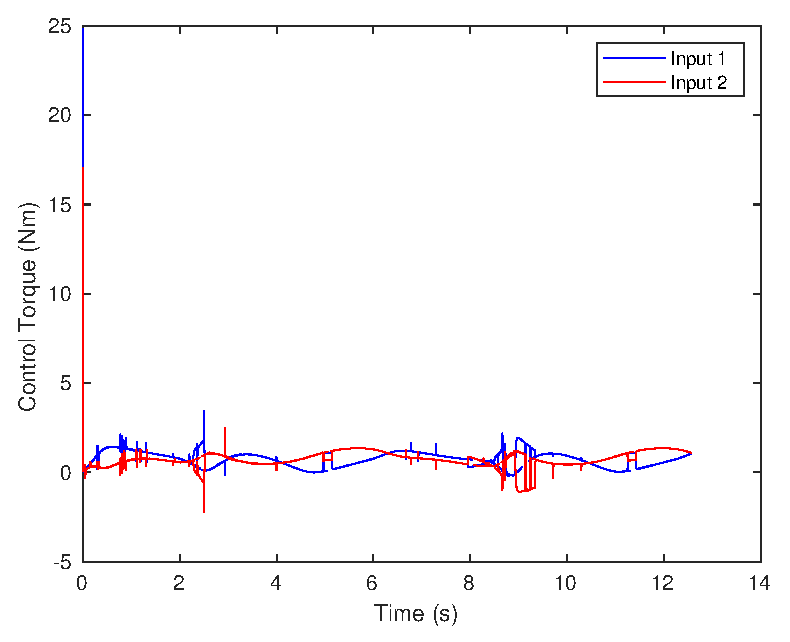
\includegraphics[width=0.7\linewidth]{./FIGS/TRACK_3}
    \caption{}
    \label{fig:track3}
  \end{subfigure}
  
  \begin{subfigure}[!t]{0.5\linewidth}
    \centering
    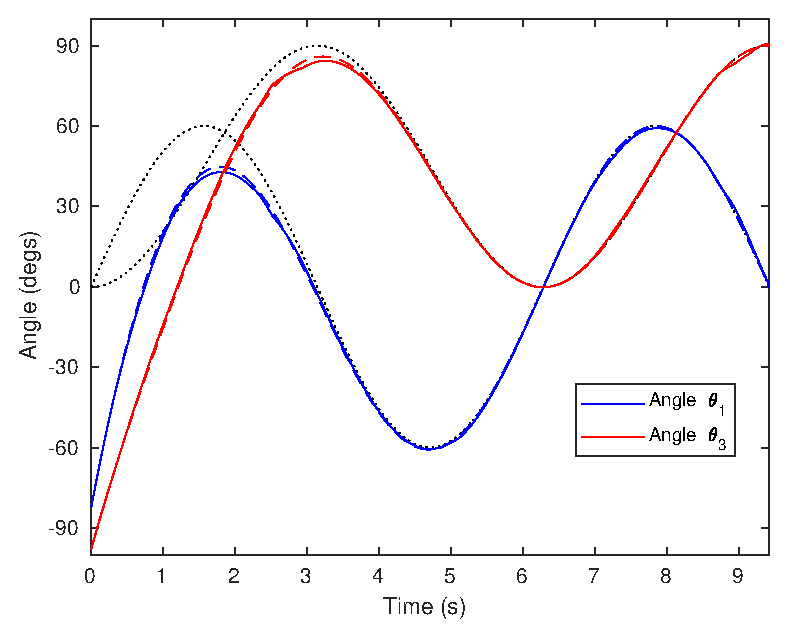
\includegraphics[width=0.7\linewidth]{./FIGS/TRACK_1}
    \caption{}
    \label{fig:track1}
  \end{subfigure}%
  \begin{subfigure}[!t]{0.5\linewidth}
    \centering
    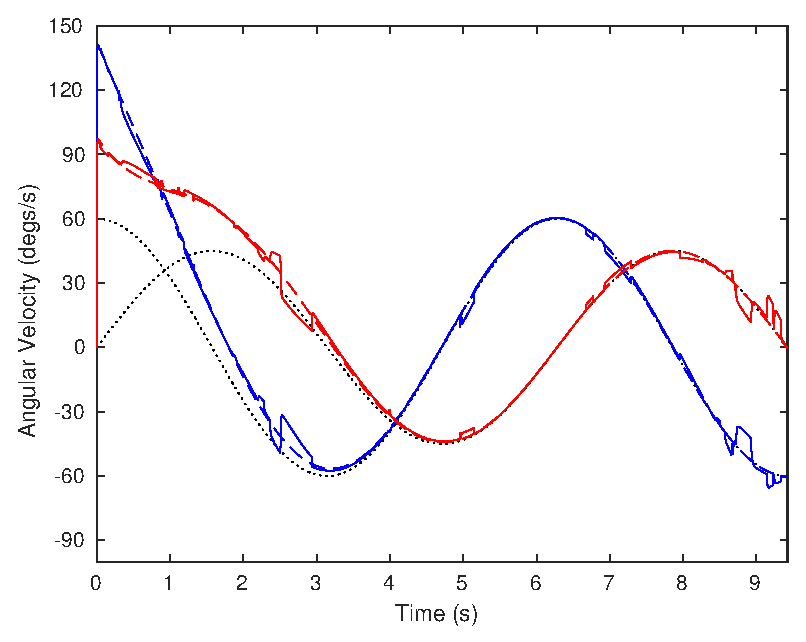
\includegraphics[width=0.7\linewidth]{./FIGS/TRACK_2}
    \caption{}
    \label{fig:track2}
  \end{subfigure}
  \caption{Tracking Control Results. (a) shows the response in the
    generalized coordinates-space, (b) shows the control torque time
    history, and (c-d) show the angular displacements and velocities
    for $\theta_1$ \& $\theta_3$ (corresponding desired configurations
    are plotted with dots). Dashed lines are simulations with the SPF;
    continuous lines are simulations with the reduced system.}
  \label{fig:tracking}
  % \setcounter{figure}{\value{mytempcntr}}
\end{figure*}

\section{Conclusions}
\label{sec:conclusions}

The procedure for developing a local reduced representation of a
Differential Algebraic System in terms of an Ordinary Differential
Equation system is presented in the context of Closed Kinematic
Chains. A Singular Perturbation Formulation of the same system is also
presented with results proving the accuracy of the formulation with
respect to the original DAE. Stability of two controllers for the
set-point regulation and tracking of such systems with fully known
parameters are presented. The stability of the controller for the
set-point case can be established with the exact model
itself. However, a full-state model has to be introduced for the proof
of the tracking controller. The presented SPF is used in the current
work to demonstrate the same. A 5-bar CKC, based on the Rice Planar
Delta Robot is used to conduct numerical simulations characterizing
(numerically) the singularities and assessing set-point \& tracking
control performances. In both the control cases, the developed
controllers are observed to show satisfactory performance.


\appendix{}

\section{Equations of Motion}
\label{sec:equations-motion}

The individual terms in the unconstrained form of the 5-bar CKC
dynamical equations of motion are given as
\begin{align}
  \bm{D}'(q') &= \begin{bmatrix} d_{11} & d_{12} & 0 & 0\\
    d_{12} & d_{22} & 0 & 0\\ 0 & 0 & d_{33} & d_{34}\\
    0 & 0 & d_{34} & d_{44} \end{bmatrix}\nonumber\\
  \bm{C}'(q') &= \begin{bmatrix} c_{11} & c_{12} & 0 & 0\\
    c_{21} & 0 & 0 & 0\\ 0 & 0 & c_{33} & c_{34}\\
    0 & 0 & c_{43} & 0 \end{bmatrix}\nonumber\\
  H'(q') &= \begin{bmatrix} h_1\\ h_2\\ h_3\\ h_4 \end{bmatrix}.
  \label{eq:eomform}
\end{align}
The individual terms of the inertia matrix are
\begin{align}
  d_{11} &= I_1+I_2+m_1c_1^2 + m_2(l_1^2 + c_2^2 +
           2l_1c_2\cos\theta_2)\nonumber\\
  d_{12} &= I_2+m_2c_2^2+m_2l_1c_2\cos\theta_2\nonumber\\
  d_{22} &= I_2+m_2c_2^2\nonumber\\
  d_{33} &= I_3+I_4+m_3c_3^2 + m_4(l_3^2 + c_4^2 +
           2l_3c_4\cos\theta_4)\nonumber\\
  d_{34} &= I_4+m_4c_4^2+m_4l_3c_4\cos\theta_4\nonumber\\
  d_{44} &= I_4+m_4c_4^2  
  \label{eq:inertterms}
\end{align}
Correspondingly, the Christoffel symbols are
\begin{align}
  c_{11} &= -2m_2l_1c_2\dot{\theta_2}\sin q_2\nonumber\\
  c_{12} &= -m_2l_1c_2\dot{\theta_2}^2\sin\theta_2\nonumber\\
  c_{21} &= m_2l_1c_2\dot{\theta_1}\sin\theta_2\nonumber\\
  c_{33} &= -2m_4l_3c_4\dot{\theta_4}\sin q_4\nonumber\\
  c_{34} &= -m_4l_3c_4\dot{\theta_4}^2\sin\theta_4\nonumber\\
  c_{43} &= m_4l_3c_4\dot{\theta_3}\sin\theta_4.
  \label{eq:csymbterms}
\end{align}
The nonlinear forcing/gravity vector terms are
\begin{align}
  h_1 &= (m_1c_1+m_2l_1)g\cos\theta_1 +
        (m_2c_2)g\cos(\theta_1+\theta_2)\nonumber\\
  h_2 &= (m_2c_2)g\cos(\theta_1+\theta_2)\nonumber\\
  h_3 &= (m_3c_3+m_4l_3)g\cos\theta_3 +
        (m_4c_4)g\cos(\theta_3+\theta_4)\nonumber\\
  h_4 &= (m_4c_4)g\cos(\theta_3+\theta_4).
  \label{eq:gravterms}
\end{align}
The loop-closure constraint equations $\phi(q')$ are
\begin{align}
  l_1\cos\theta_1 + l_2\cos(\theta_1+\theta_2) -
  l_3\cos(\theta_3+\theta_4&)\nonumber\\
  - l_4\cos\theta_4 - c &= 0\nonumber\\
  l_1\sin\theta_1 + l_2\sin(\theta_1+\theta_2) -
  l_3\sin(\theta_3+\theta_4&)\nonumber\\
  - l_4\sin\theta_4 &= 0.
  \label{eq:lcconst}
\end{align}
  
\bibliographystyle{IEEEtran}
\bibliography{IEEEabrv,Refs}
\end{document}
%%% Local Variables:
%%% mode: latex
%%% TeX-master: t
%%% End:

(setq buffer-auto-save-file-name buffer-file-name)